
\documentclass[11pt]{asu}

\usepackage[]{graphics}
\usepackage{graphicx}
\usepackage{setspace}
\usepackage{lscape}
\usepackage{rotating}
\usepackage{listings}
\usepackage{url}
\usepackage[dvipsnames]{xcolor}
\usepackage{soul}
\usepackage{courier}
\usepackage{csquotes}
\usepackage{fixltx2e}
\usepackage{xinttools}
\usepackage{physics}
\usepackage{multirow}
\usepackage{verbatim}
\usepackage{float}
\usepackage{units}
\usepackage{calc}
\usepackage[]{algorithm2e}
\usepackage[toc,page]{appendix}

\newcounter{bitindex}

\clubpenalty=5000
\widowpenalty=5000
\renewcommand\lstlistlistingname{List of Listings}
\setlength{\belowcaptionskip}{.25in}

\definecolor{myblue}{rgb}{0,0,0.6}
\lstset{language=python,
	numberstyle=\footnotesize,
	basicstyle=\ttfamily\footnotesize,
	commentstyle=\color{myblue},
	morekeywords={with, as},
	numbers=left,
	stepnumber=1,
	frame=single,
	breaklines=true,
  showstringspaces=false
}


% define tag textSq for visualizing quantum gates
\makeatletter
\def\textSq#1{%
\begingroup% make boxes and lengths local
\setlength{\fboxsep}{0.3ex}% SET ANY DESIRED PADDING HERE
\setbox1=\hbox{#1}% save the contents
\setlength{\@tempdima}{\maxof{\wd1}{\ht1+\dp1}}% size of the box
\setlength{\@tempdimb}{(\@tempdima-\ht1+\dp1)/2}% vertical raise
\raise-\@tempdimb\hbox{\fbox{\vbox to \@tempdima{%
  \vfil\hbox to \@tempdima{\hfil\copy1\hfil}\vfil}}}%
\endgroup%
}
\def\Sq#1{\textSq{\ensuremath{#1}}}%
\makeatother

%inline code command, using courier font
\definecolor{light-gray}{gray}{0.90}
\newcommand{\plaintext}[1]{\texttt{#1}}
\newcommand{\code}[1]{\begin{verbatim}[#1]\end{verbatim}}

\title{A Simulation of the BB84 Quantum Key Exchange Protocol}
\degree{Bachelor of Science}
\department{Computer Science}
\gradmonth{December}
\gradyear{2019}
\author{Andrew Thorp}  
\thesischair{Raghuveer Mohan, Ph.D.}
\thesismemberone{Chad Waters, M.Sc.}
\thesismembertwo{Raghuveer Mohan, Ph.D.}
\deptchair{Rahman Tashakkori, Ph.D.}
\dean{Dean}

\begin{document}
	\begin{preliminary}
		\maketitle
        \makecopyright
        \begin{acknowledgement}

\end{acknowledgement}

        \begin{abstract}
 Hello world!
\end{abstract}

		\tableofcontents
        %\listoftables
        \listoffigures
        \lstlistoflistings
	\end{preliminary}

	\newlinestretch{2}

		\begin{doublespace}
	    \chapter{Introduction}
\label{chap:introduction}

% Establish a presidence 
Personal computers have been developed to a point where those unfamiliar with computer science theory might conclude there is nothing computers cannot do.
While this is an understandable conclusion, it has been proven that there is a limit to the types of computation our ``classical computers", what we today consider general purpose computers, can perform \cite{linz}.
In the last few decades however, the field of quantum mechanics and quantum computing have advanced to the point where primitive operations are now possible in the quantum sphere.
Just this year Google claimed to acheive ``quantum supremacy" in an experiment in which they performed a computation, using a quantum computer, in under five minutes. 
Google estimated that the same computation would take a state-of-the-art super computer 10,000 years to complete \cite{quantum_supremacy}. 
While quantum computers are not general purpose, they can solve NP-Hard and exponentially complex problems in polynomial time or better \cite{TODO}.
This breakthrough in computability will change the way information is stored, secured, and created.


% State the problem
Currently, encryption protocols ensure the integrity of data and identities are trusted.
One such protocol is the the widly adopted Diffe-Hellman protocol, which relies on the historic difficulty of factoring large prime numbers for security \cite{qc:agi}.
The protocol works by using a public and private key pair for each participating party.
Data encrypted using a key (usually a public key) can then be decrypted using the private key.
For example, a person's public and private keys are mathematically related to their private key, and it requires factoring large prime number to derive the private ky from the public key, which is comutationally infeasible with a classical computer.
Quantum computers however, are able to do this in only polynomial time complexity \cite{doi:10.1137/S0036144598347011}.
This development, combined with the growing power of quantum computers, gives rise to security concerns to the Diffe-Hellman protocol in the future.

% Mention the solution
One such development was the BB84 quantum key distribution protocol.
There are many encryption protocols in use today, such as the Diffe-Hellman key exchange protocol (KEP), each of which provide their own various security measures.
The BB84 protocol allows two parties to co-generate a disposable encryption key which can be used once to encrypt then decrypt data, and be discarded after use.
This type of key is known as a one-time-pad, and it gets its security from being disposable; data patterns are harder to identify the fewer times data is encrypted using a key \cite{TODO}.
The BB84 protocol allows for detection of an eavesdropper durring key generation, allowing both parties to abort the key generation process before any encrypted messages are transmitted \cite{qcftgu}.
This thesis presents a peer to peer simulation of the BB84 quantum quantum KEP, and serves as an introduction to programming in the quantum computing paradigm using simulaqron, a quantum network simulator \cite{simulaqron}.

% Describe the thesis' coontribution to the problem

% Describe the thesis content

Chapter~\ref{chap:background} of the thesis provides background information on encryption protocols, the quantum computation paradigm, and other background information related to the BB84 protocol. 

Chapter~\ref{chap:bb84} details the BB84 protocol in its steps, as well as discusses the guarantees the protocol provides the user.

Chapter~\ref{chap:implementation} describes the library.
This describes not only the documentation for the library but also how it can be used.

Chapter~\ref{chap:conclusion} summarizes this simulator and its potential applications, as well as discussing possible future work to improve upon it.


	    8p\chapter{Preliminaries}
\label{chap:background}

% Describe what we need to understand to move forward
In this chapter, we discuss the preliminaries of encryption and quantum computation, the two ideas key to understanding the BB84 quantum KEP.


\section{Encryption}
Consider two parties, Alice and Bob, trying to communicate through a channel.
If the channel is insucure, a malicious third party, Eve, can listen and eavesdrop on the communication.
Encryption helps to make the communication more secure, by obscuring data such that an eavesdropper cannot gain any information by intercepting communication \cite{encrypt}.

\begin{figure}[htp]
\centering
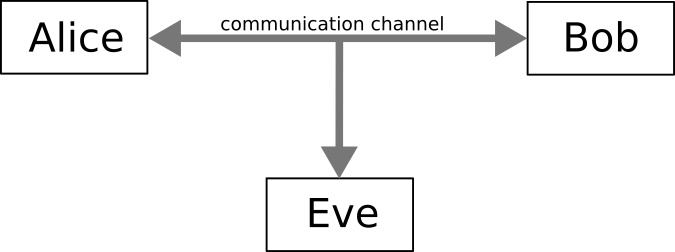
\includegraphics[scale=0.4]{images/classical_communication.png}
\caption{Alice and Bob communicate over an insecure channel with an eavesdropper, Eve}
\label{foo bar}
\end{figure}

In practice, information is encrypted by manipulating the data according to some encryption algorithm.
The goal of a good encryption algorithm is simple: allow the sender and receiver to access the information, but make the data useless to anyone else.
In order to allow for information to be decrypted by the receiver, the algorithm must be reversible with the use of a secret key, also known as the encryption key.
The basic encryption process is as follows:

\begin{itemize}
\item A sender, Alice, composes a message, referred to as the plaintext.
\item Alice encrypts the plaintext into cyphertext using some encryption algorithm and an encryption key.
\item Alice then sends the cyphertext to the receiver, Bob.
\item Bob uses the encryption key to decrypt the cyphertext into plaintext.
\item Note that the plaintext was never transmitted over the network.
\end{itemize}

Encryption appears in two general forms: symmetric and asymmetric, each with their own benefits and drawbacks. 


\subsection{Symmetric Encryption}
% Symmetric Encryption
Symmetric encryption is an encryption method in which both the sender and receiver, Alice and Bob respectively, use the same key.
\begin{figure}[htp]
\centering
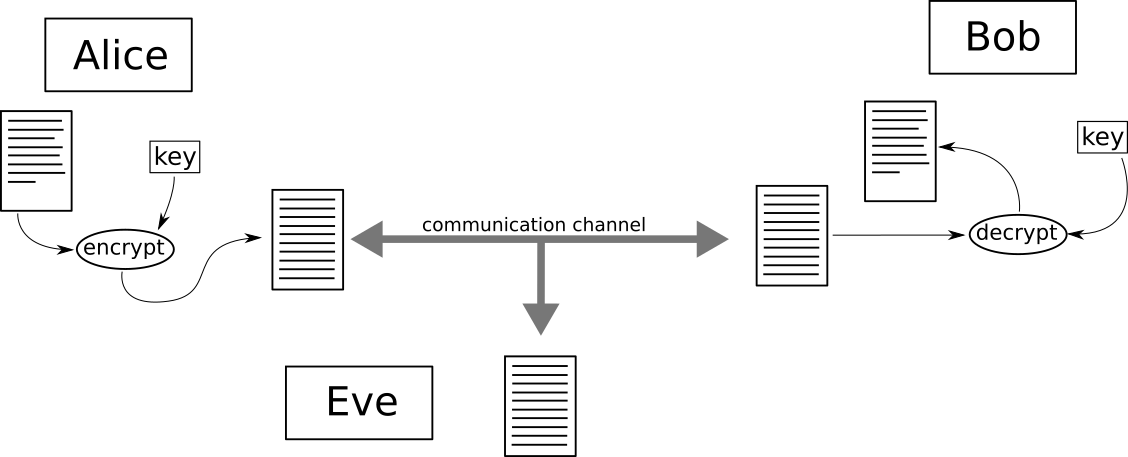
\includegraphics[scale=0.350]{images/symmetric_ecryption.png}
\caption{Alice and Bob symmetrically encrypt and decrypt a message}
\label{}
\end{figure}
While symmetric encryption is the oldest form of encryption, being used for over 4000 years, it does have a major drawback -- the key distribution problem: if Alice and Bob are separate parties (as in the case of secure message transmission), they must exchange their key beforehand using a secure channel \cite{cryptography}.
If an eavesdropper, Eve, were to intercept the key in transit, then the encryption is compromised and there is not necessarily any way for Alice or Bob to know.

% Talk about AES encryption and/or stream cyphers

% One Time Pad in depth
A One-Time-Pad (OTP) is a symmetric key that is used only once.
The OTP, as the name suggests, is discarded after a singe message has been sent, and the OTP is usually the same length as the message it encrypts.
This allows bit-wise encryption techniques, such as parity manipulation, to add the the security of the key and ensures that common frequency hacking techniques are not possible \cite{cryptography}.
In order to make the OTP truly secure, the bits used must be generated using a true-random number generator to avoid a malicious party guessing the pad.
Data is encrypted using a OTP with the following bitwise operation:
\begin{center}
\begin{tabular}{rc}
Plaintext: & $X = \{x_0, x_1, ..., x_n\}$ \\
OTP:  & $P = \{p_0, p_1, ..., p_n\}$  \\
Cyphertext:  & $Y = \{y_0, y_1, ..., y_n \}$\\
where  & $y_i = (x_i + p_i) \mod 2 $\\
\end{tabular}
\end{center}

For example, in binary:

\begin{center}
\begin{tabular}{rc}
Plaintext: &  \code{ 0 1 0 0 1 0 1 0} \\
OTP: &        \code{ 0 1 1 0 1 0 0 1} \\
Cyphertext: & \code{ 0 0 1 0 0 0 1 1} \\
\end{tabular}
\end{center}

To decrypt the cyphertext using the OTP, you simply apply the same opperation:

\begin{center}
\begin{tabular}{rc}
Cyphertext: & \code{ 0 0 1 0 0 0 1 1} \\
OTP: &        \code{ 0 1 1 0 1 0 0 1} \\
Plaintext: &  \code{ 0 1 0 0 1 0 1 0} \\
\end{tabular}
\end{center}
Under the proper conditions, a OTP is considered to be ``perfect encryption", and is only susceptible to brute force attacks, where one has to try every possible combination of the secret key, which is computationally infeasible \cite{cryptography}.
% One Time Pad caveats
However OTPs suffer from the same issue as all symmetric encryption protocols, the key distribution problem.
In the case of the OTP, not only does one encryption key have to be distributed, a unique key must be distributed for each message, making it highly impractical in most cases.

\subsection{Asymmetric Encryption}
% Asymmetric encryption
Asymmetric encryption, also known as public-key cryptography, on a classical computer, is the process of encrypting data using one key in such a way that it can be decrypted using a different key.
In effect, Alice can encrypt a message using a key that is publicly accessible, and the message can only be decrypted by Bob, who has the secret key corresponding to the public key used.
This method requires a key to be compromised of two parts, a public and private key-pair: $k = (k_{pub}, k_{priv})$ where $k_{pub} = f(k_{priv})$ \cite{cryptography}.

% Diffie Hellman in depth
The Diffie-Hellman KEP was the first asymmetric KEP to be proposed, and is still widely used in various forms today. 
It is performed as follows:

\begin{enumerate}
\item The sender and receiver, Alice and Bob respectively, establish a line of communication.
\item Some large prime $p$ and an integer $\alpha \in \{2,3,4,...,p-2\}$ are shared between Alice and Bob.
\item Alice and Bob each compute their own private keys, $a$ and $b$, respectively. $$k_{priv,A} = a \in \{2,3,4,...,p-2\}$$
\item Alice sends Bob her public key $A = \alpha^a \mod p$.
\item Bob sends Alice his public key $B = \alpha^b \mod p$. 
\item Alice computes a session key $k_{AB} = B^a \mod p$.
\item Bob computes a session key $k_{AB} = A^b \mod p$. 
Because $(\alpha^a)^b = (\alpha^b)^a = \alpha^{ab}$, both Alice and Bob's computations result in the same session key despite never knowing each other's private keys. 
\end{enumerate}

This method is cryptographically secure due to the Discreet Logarithm Problem (DLP), finding $x$ such that $B = \alpha^x \mod p$. 
This problem is computationally not feasible to solve using classical computers; although it has never been shown to be NP-Hard, nor has it been shown to be polynomial time solvable \cite{Shor_1997}.
Although these techniques are currently secure, they become easy to solve in the quantum space.

\section{Quantum Computation}

% Basic properties
Just as classical computation involves bits, quantum computation is computation using quantum bits, qubits, which are usually denoted using ``bra-ket" notation as $\ket{\psi}$ \cite{qc:agi}.
A ket is simply a representation of a vector, and in this case the vector is the ``state-vector" of the qubit, as further explained.
Similar to classical bits having the value 0 or 1, qubits' state can be the analogous $\ket{0}$ or $\ket{1}$.
These states will be used as binary, just like 0 and 1, for computation.
%	State
It is commonly said that while a classical bit exists in either the state 0 or 1, qubits can exist in both $\ket{0}$ and $\ket{1}$ at once.
There is an element of truth in this, but a more accurate description would be that as a qubits state-vector exists in a 3-dimensional space, and it can point somewhere in between the states $\ket{0}$ and $\ket{1}$. 
This state-vector is described as a linear combination $\ket{\psi} = \alpha\ket{0} + \beta\ket{1}$, where $|\alpha|^2 + |\beta|^2 = 1$, and $\alpha$ and $\beta$ are referred to as the amplitude of probability for their respective kets.

%	Measurement
Just as a computer can read the value of a classical bit, we can read, or``measure", a qubit.
The measurement is performed against two states, $\ket{0}$ and $\ket{1}$, and upon measurement the qubits state collapses to one of the two values.
The probability with which a vector will collapse into one of two states is the square of the amplitude for that state.
It is unknown exactly what causes the superposition to collapse, but it has been derived from empirical observations and is the single most important property of quantum mechanics \cite{qc:agi}.
For example, consider the qubit $\ket{\psi} = \frac{1}{\sqrt{3}}\ket{0} + \sqrt{\frac{2}{3}}\ket{1}$.
The probability that $\ket{\psi}$ will be $\ket{0}$ when measured is $(\frac{1}{\sqrt{3}})^2$, or $\frac{1}{3}$.
Any qubit or state-vector is defined using this vector formula.
If $\ket{\psi}$ is a linear combination of $\ket{0}$ and $\ket{1}$, and neither amplitudes are zero, the qubit is said to be in a superposition of $\ket{0}$ and $\ket{1}$.
Superposition is one of the fundamental properties of quantum computation \cite{qc:agi}. 

We use quantum operators called gates to manipulate $\alpha$ and $\beta$ probabilities.
For example, the Hadamard Gate, or H gate, performs what is called a "quarter turn"; it maps $$\ket{\psi} = \ket{0} \rightarrow \textSq{H} \rightarrow \ket{\psi} = \frac{1}{\sqrt{2}}\ket{0} + \frac{1}{\sqrt{2}}\ket{1}$$  $$\ket{\psi} = \ket{1} \rightarrow \textSq{H} \rightarrow \ket{\psi} = \frac{1}{\sqrt{2}}\ket{0} - \frac{1}{\sqrt{2}}\ket{1}$$ \cite{qc:agi}.
Since after the H gate is applied $\alpha$ and $\beta$ both equal $\frac{1}{\sqrt{2}}$, and ${(\frac{1}{\sqrt{2}})}^2 = \frac{1}{2}$, if we measure $\ket{\psi}$ in this state it would collapse to $\ket{0}$ and $\ket{1}$ with equal probability. 
It is worth noting this is one way to create a true-random number generator.

%	Bases
Because the state vector exists in a 3D state space, we do not necessarily have to measure against $\ket{0}$ and $\ket{1}$, in fact we can measure against any two vector values that are opposite each other on the unit circle. 
A set of vectors to measure against is known as a basis, and there are many possible bases. 
The set $\{\ket{0},\ket{1}\}$ is known as the standard basis or computational basis, as it is analogous to classical bits \cite{qcftgu}.
Another common basis is the Hadamard Basis, which is denoted $\ket{+} = \frac{1}{\sqrt{2}}\ket{0} + \frac{1}{\sqrt{2}}\ket{1}$ and $\ket{-} = \frac{1}{\sqrt{2}}\ket{0} - \frac{1}{\sqrt{2}}\ket{1}$.
The H gate will put $\ket{0} \rightarrow \ket{+}$ and $\ket{1} \rightarrow \ket{-}$, but it will also revert the Hadamard basis into the standard basis: $\ket{+} \rightarrow \ket{0}$ and $\ket{-} \rightarrow \ket{1}$.

Because the standard basis and the Hadamard basis are perpendicular to each other they are referred to as orthonormal bases.
That is to say if a $\ket{\psi} = \ket{+}$ or $\ket{\psi} = \ket{-}$ then it will have a 50\% change of being $\ket{0}$ or $\ket{1}$ if measured in the standard basis, and vice-versa \cite{qc:agi}. 

\begin{figure}[H]
\centering
\begin{tabular}{cc|cccc}
	&&\multicolumn{4}{|  c }{Measured value}  \\
	   &       &$ \ket{0}$ & $\ket{1}$ & $\ket{+}$ & $\ket{-}$\\ \hline
	\multirow{4}{*}{Qubit state} &$\ket{0}$ & $100\%$   & $0\%$     & $50\%$    &  $50\%$  \\
	&$\ket{1}$ & $0\%$     & $100\%$   & $50\%$    &  $50\%$  \\
	&$\ket{+}$ & $50\%$    & $50\%$    & $100\%$   &  $0\%$   \\
	&$\ket{-}$ & $50\%$    & $50\%$    & $0\%$     &  $100\%$ \\
\end{tabular}
\caption{The probability of measuring a qubit from one basis state into another}
\end{figure}

In effect, if you have a vector in one orthonormal basis it is useless if measured in another orthonormal basis.
Further, since the vector state changes when measured, if a value is encoded in one orthonormal basis, that information is destroyed by measuring in another orthonormal basis \cite{qcftgu}. 

% Guarantees
% 	Copy-ability
Another crucial property of qubits is that they cannot be cloned.
It is impossible to have an operator that clones the state of an input qubit into an output qubit without knowing the basis of the input \cite{qc:agi}.
This property proves crucial in the BB84 protocol, as explained in Chapter~\ref{chap:bb84}.

Using these properties and others, it has been shown that quantum computers can solve the DLP on an $n$-bit number in only $O(n^2\log n \log \log n)$ time \cite{MikeAndIke}.
Therefore, the popularity of quantum computers poses a serious threat to the securities of the Diffie Hellman KEP and asymmetric encryption.
The BB84 protocol is a quantum key distribution (QKD) protocol that allows two parties to co-create a shared key, using a verifiably secure channel, that can then be used to symmetrically encrypt messages.

	    \chapter{Quantum Key Distribution}
\label{chap:bb84}

% Talk about quantum key distribution
Quantum computers have been shown to solve the mathematical problems that make our encryption secure.
Although symmetric encryption is much less effected by this, it is not commonly used due to the key distribution problem \cite{cryptography}.
One potential solution to this issue is the use of Quantum Key Distribution (QKD) which is the application of quantum mechanics and quantum computing properties in a key distribution protocol that is provably secure \cite{MikeAndIke}.
It allows for two parties to securely generate a symmetric key.
In this chapter, we look at the BB84 quantum key exchange protocol that uses principles of quantum mechanics to exchange encryption keys between two parties, Alice and Bob.
The encryption key is exchanged through a quantum channel in the form of qubits.
An eavesdropper listening in on this communication cannot obtain any information without disturbing the qubits and measuring them, which introduces noise to the signal since the basis is unknown. 
This means the security of the BB84 protocol comes from the fundamental laws of quantum physics \cite{MikeAndIke}.

% Introduce protocol
\section{The BB84 Protocol}

\begin{figure}[htp]
	\centering
	\fbox{\begin{minipage}{41em}
	\begin{center}
		\textbf{BB84}
	\end{center}
	\begin{enumerate}
	\item  Alice and Bob connect via quantum network simulator.
    \item  Alice generates $N$ random bits, where $N \geq 3k$, $k$ = desired key size
    \item  Alice encodes the bits into qubits, randomly choosing to encode using one of two orthonormal bases.
    \item  Alice sends the qubits to Bob.
    \item  Bob measures each qubit, choosing to use one of the two selected bases at random.
    \item  Bob sends a bitvector of his chosen bases to Alice over a classical channel.
    \item  Alice responds with a bitvector showing which of Bob's bases were correct.
    \item  Alice and Bob discard all qubits that were measured in the wrong basis.
    \item  Bob sends Alice some number of the measured values to ensure the key was received without any interference.
    \item Alice responds with whether or not the exchanged values were correct.
    \item If there were no errors in the compared bits, the bits that were exchanged are discarded by both parties, and the rest of the bits are used as the key.
    \end{enumerate}
	\end{minipage}}
\caption{A formal definition of the BB84 Quantum Key Distribution Protocol}
	\label{fig:BB84}
\end{figure}

In 1984 Charles Bennett and Gilles Brassard proposed the first quantum key distribution protocol, the BB84 \cite{qc:agi}.
The protocol allows two parties communicating over a public classical channel, such as the internet, and a public quantum channel to securely generate a shared encryption key for symmetric encryption.

To start the quantum key exchange, Alice randomly generates two bit sequences, $a$ and $b$, of length at least $N = 4l$ bits each, where $l$ is the intended key length. 
Alice then encodes $a$ into a block of $N$ qubits, $\ket{\psi}$.
This is done using two bases; in our case, the standard basis and Hadamard basis.
The basis chosen for encoding each bit in $a$ is determined by the corresponding bit in $b$, with $b_i = \{0 or 1\}$ where $0 \Rightarrow$ standard basis and $1 \Rightarrow$ Hadamard basis.
Thus, each qubit is in either the standard basis or the Hadamard basis, and is in one of four states shown in figure ~\ref{fig:possible_states}.
\begin{figure}[htp]
\centering
\begin{tabular}{|c|c|c|}
\hline
$a_i$ & $b_i$ & $\ket{\psi_i}$ \\ \hline
0 & 0 & $\ket{0}$ \\ \hline
1 & 0 & $\ket{1}$ \\ \hline
0 & 1 & $\ket{+}$ \\ \hline
1 & 1 & $\ket{-}$ \\ \hline
\end{tabular}
\caption{The four possible states of a qubit in a BB84 encoded string}
\label{fig:possible_states}
\end{figure}
Now Alice has the qubits encoding $a$, $\ket{\psi}$, the bases of which are determined by $b$.
Alice sends each qubit to Bob using a public quantum channel.
When Bob has received each qubit he can assemble the full qubit block $\ket{\psi}^\prime$.
Assuming a perfect quantum channel and no eavesdropping, there should not be any disturbance or noise in the communication: $\ket{\psi} = \ket{\psi}^\prime$.
Once Bob has received all qubits, he measures each qubit in $\ket{\psi}^\prime$ into a bit sequence $a^\prime$ by randomly choosing a basis of measurement for each bit.
The bases chosen are stored in a bit sequence $b^\prime$.
Bob then informs Alice that he has measured all the received qubits.
Because there is a 50\% chance that Bob will choose an incorrect basis for measurement for each qubit, and a 50\% probability of measuring the correct value using the wrong basis, Bob has measured 75\% of the qubits correctly, on average (figure ~\ref{fig:possible_measurements_no_eve}).
\begin{figure}[htp]
	\centering
	\begin{tabular}{|r|c|c|c|c|c|c|c|c|}
		\hline
		Encoded value  & 0 & 0 & 0 & 0 & 1 & 1 & 1 & 1 \\ \hline
		Encoded basis  & 0 & 0 & 1 & 1 & 0 & 0 & 1 & 1 \\ \hline
		Measured basis  & 0 & 1 & 0 & 1 & 0 & 1 & 0 & 1 \\ \hline
		Measured value & 0 & $\nicefrac{0}{1}$& $\nicefrac{0}{1}$ & 0 & 1 & $\nicefrac{0}{1}$ & $\nicefrac{0}{1}$ & 1\\
		\hline
	\end{tabular}
	\caption{Exhaustive list of encoding and measurement of a single qubit between Alice and Bob}
	\label{fig:possible_measurements_no_eve}
\end{figure}
While 75\% of the bits are measured correct on average, an average of 50\% are measured in the correct basis; those qubits are  guaranteed to be measured correctly.
Note that Alice has ($a$, $b$) and Bob has($a^\prime$ $b^\prime$), but they each do not know the others $a$ and $a^\prime$.
Alice and Bob now exchange the bases they each used, $b$ and $b^\prime$, respectively.
Alice and Bob both discard every bit that was encoded and measured using different bases: bit $i$ is discarded from $a$ and $a^\prime$ if $b_i \neq b^\prime_k$.
They store the remaining bits from $a$ and $a^\prime$ into a new bit sequence, $k$ and $k^\prime$, respectively.
Alice and Bob now each have the same key, $k = k^\prime$.
They each exchange some number of bits from $k$ to verify there was no error in their key generation.
If the exchanged bits are identical, then Alice and Bob can confirm with high probability that there was no eavesdropper, and that they key is secure \cite{MikeAndIke}.
They can now use the key for symmetrically encrypted communication, or even as a OTP.

% Discuss eavesdropping
If an eavesdropper, Eve, were to attempt to listen in on the conversation, not only would they not be able to gain any useful information from the qubits, since she does not know the basis at which the qubits are encoded, nor can she duplicate the qubits. 
Therefore the only strategy she has is to perform a ``man-in-the-middle" attack, in which Eve impersonates Bob to Alice and Alice to Bob \cite{qc:agi}.

To eavesdrop on the communication, Eve listens on the quantum channel and waits for Alice to transmit qubits.
As Alice sends Bob the qubits over the quantum channel Eve intercepts each qubit, forming her own qubit block $\ket{\psi}^\prime$.
With the qubits now in Eve's possession, she attempt to measure the qubits or clone them.
However, as previously shown, this would introduce noise to the signal, reducing Bob's correct average measurement percentage from 75\% to 62.5\%, leaving only 25\% of the qubits measured in the same basis used during encoding.
\begin{figure}[htp]
	\centering
	\begin{tabular}{|c|c|c|c|c|}
		% Table headers
		\hline
		$\textrm{Basis}_{Alice}$ & $\textrm{Basis}_{Eve}$ &$\textrm{Basis}_{Bob}$ & Percent Correct & In Final Key\\ \hline
	%	Ab  Eb  Bb  c       a       
    	0 & 0 & 0 & 100\% & 1 \\ \hline		
    	0 & 0 & 1 &  50\% & 0 \\ \hline		
    	0 & 1 & 0 &  50\% & 1 \\ \hline		
    	0 & 1 & 1 &  50\% & 0 \\ \hline		
    	1 & 0 & 0 &  50\% & 0 \\ \hline		
    	1 & 0 & 1 &  50\% & 1 \\ \hline		
    	1 & 1 & 0 &  50\% & 0 \\ \hline		
    	1 & 1 & 1 & 100\% & 1 \\ \hline		
	\end{tabular}
	\caption{Exhaustive list of encoding and measurement of a single qubit between Alice and Bob with an eavesdropper}
	\label{fig:possible_measurements_eve}
\end{figure}
As can be seen in figure~\ref{fig:possible_measurements_eve}, when there is an eavesdropper, half of the bits kept in the generated key are measured in an incorrect basis by at least one party.
This means, on average, 25\% of the bits in $k^\prime$ are incorrect.
When Alice and Bob exchange some bits to verify their correctness, even if only four bits are compared they both will, on average, detect that the qubits were maliciously measured during transmission, at which point Alice and Bob can abort communication \cite{MikeAndIke}. 

In practice this protocol can be implemented using polarized photons as qubits, which can be sent between Alice and Bob using fiber optics.
The data is encoded into the photons using the angle of the polarization since polarization can act as a qubit \cite{qc:agi}.
In this case the bases for encoding data are the standard basis, $(\ket{0}, \ket{1}) = (\ket{\rightarrow}, \ket{\uparrow})$, and the Hadamard basis, $(\ket{+}, \ket{-}) = (\ket{\nearrow}, \ket{\nwarrow})$.
However all that is required to perform any QKD protocol is the ability to communicate qubits over a public channel with a very low error rate \cite{MikeAndIke}.
      	\chapter{The BB84 Simulation Library}
\label{chap:implementation}


        \chapter{Conclusion}
\label{chap:conclusion}

\section{Summary}
The BB84 protocol is nothing new, however as quantum computers become more powerful and QPUs become more accessible, the ability to program in the quantum paradigm is becoming more important.
Using the BB84 as an example we have shown that the BB84 works not only in theory but in practice.
The BB84 library is an empirical example of the availability and simplicity of today's quantum computation libraries power and accessibility.
BBchat can be used a secure chat client, and functions as an example for how one might integrate a QKD protocol into their own software.

Though there is still much development to be done in the quantum paradigm, such as true-quantum networking, there have already been great strides in the accessibility of quantum computation for computer programmers.

\section{Future Work}
The BBChat messenger works between two local clients and a locally running simulaqron server.
Although this works well for a proof of concept, a crucial element to distribute the software is configuring remote support for messaging. 
Allowing someone the ability to specify the url of both the server and the message recipient.
Along these same lines, the messenger TUI could be re-arranged to make it more user friendly.

Currently the program only supports the BB84 protocol, but there are several QKD protocols that could be used.
One such protocol is the B92, which is comparable to the BB84, but is designed differently. 
Unlike the BB84, which encodes qubits using randomly selected basis, the B92 encodes each bit in the key using only two states, depending on the value of that bit: $0 \rightarrow \ket{0}$ and $1 \rightarrow \ket{+}$ \cite{qc:agi}.
As potential future work, one could simulate the B92 quantum protocol using the same libraries.

Finally, since simulaqron does not currently support a true QPU backend, it would be important to create one \cite{simulaqron}.
Doing so could verify the BB84 further, allowing further research into parameter adjustment to account for noise and the true-randomness of quantum computers. 
This would be non-trivial, since current QPUs do not support persistent qubits.
One idea however, would be to enqueue all quantum gates as they are called, and dequeue all enqueued gates upon measurement, calling the QPU API to perform each operation as it is dequeued, and returning the final measurement after all gates have been executed.
Using this technique, the QPU does not have to store any information about the state of a qubit, as the qubit does not truly exist until it is measured.

		\end{doublespace}

	\newpage
    \newlinestretch{1}
	\addcontentsline{toc}{chapter}{bibliography}
	\bibliography{bibliography} 
    \bibliographystyle{plain}
\end{document}
